\chapter{État de l’art}

Les circonstances environnementales, sociétales et géopolitiques de notre planète
font que nous avons besoin d'optimiser notre consommation d'énergie.


\section{Augmentation des besoins en énergie}

Nous faisons face à une augmentation massive de la population sur Terre.
Jusqu'en 1950, sa variation fut assez lente : nous passions de 1.7 milliards d'êtres humains
en 1900, 2.0 milliards en 1930, 2.5 milliards en 1950.

Nous sommes aujourd'hui 7.5 milliards d'êtres humains en 2020. Cet emballement démographique s'explique
par plusieurs vecteurs.

Tout d'abord une révolution des conditions sanitaires et de l'espérance de vie. Autrefois la population
était naturellement régulée par des crises de surmortalité : épidémies, famines, catastrophes naturelles\dots
Ces facteurs sont aujourd'hui mieux maîtrisés par l'évolution de la médecine, de la surproduction et de l'entraide des peuples.
Le taux de natalité est resté le même malgré la diminution du taux de mortalité à la naissance, ne commençant à
diminuer progressivement qu'à partir des années 1970.

% Augmentation grandissante d'année en année
\begin{SCfigure}[][h]
  \centering
  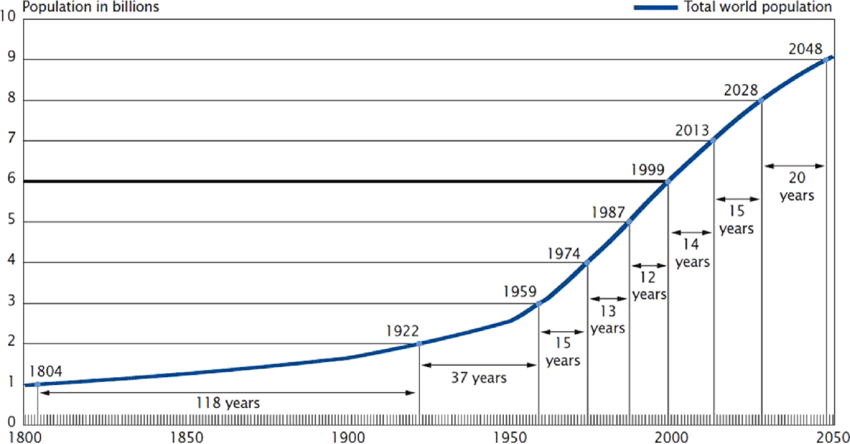
\includegraphics[scale=0.35]{media/WorldPopulation.png}
  \caption{
      Population sur Terre\newline
      \tiny{Source:\newline
        \url{https://www.researchgate.net/figure/World-Population-1800-2050-6_fig1_321996838}
      }
  }
  \label{fig:capita_energy}
\end{SCfigure}

Les guerres sont encore nombreuses mais moins mortelles que durant la première moitié du XXe siècle,
notamment en raison de la pression nucléaire. L'économiste Max Roser a calculé le taux de décès dus aux
conflits militaires par rapport à la population mondiale depuis les années 1400 (schéma A1 en annexe).
Ce taux est en chute depuis les années 2000.


Nous avons donc une population qui grossit de plus en plus chaque année.
De ce fait, les besoins en énergie de la population mondiale croient naturellement, mais cela ne fait pas tout.
L'évolution de la condition de vie sur Terre a fortement progressé suite aux découvertes réalisées durant les guerres.
Les foyers s'équipent d'appareils électroménagers augmentant leur confort, puis d'ordinateurs et d'Internet.
Nous faisons face ces deux dernières décennies à une révolution technologique avec des appareils et une consommation de services
demandant toujours plus d'éléctricité pour fonctionner.

La mondialisation connectant nos continents est aussi un facteur de poids dans la consommation de tous types de carburants.

Cette évolution de la consommation en énergie pour chaque individu est décrite par le schéma \ref{fig:capita_energy}.

\begin{SCfigure}[][h]
  \centering
  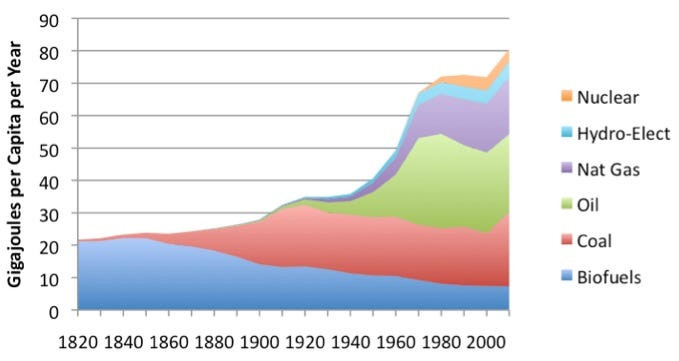
\includegraphics[scale=0.35]{media/world_per_capita_energy.jpeg}
  \caption{
      Consommation d'énergie par personne\newline
      \tiny{Source:\newline
        \url{https://www.businessinsider.com/a-worrying-look-at-world-energy-consumption-since-1820-2012-3?IR=T}
      }
  }
  \label{fig:capita_energy}
\end{SCfigure}


\section{Guerre de l'énergie}
\vskip -15pt

Le concept de la guerre est toujours le même depuis des millénaires : prendre posséssion des
ressources de l'autre pour son propre avantage.

Nous pouvons citer quelque types de guerre qui mettent a profit la faiblesse des uns
pour enrichir les plus forts :

\begin{itemize}
  \item la délimitation des territoires % ont toujours été source de conflits entraînant
  % des guerres se traduisant par la perte de vies humaines.
  \item les consommables comme les ressources agricoles ou épices
  \item les connaissances et technologies
  \item les sources énergétiques
\end{itemize}

La guerre est bien plus rare de nos jours, de nombreuses instances telle que l'ONU ou bien les
contrats commerciaux ont rendu les conflits directs moins rentables.

Aujourd'hui, les foyers de tensions n’ont pourtant pas disparus pour autant.
Ce sont essentiellement les mêmes depuis trente ans et ont tous un point commun,
ils possèdent du pétrole en sous-sol.

Le Golfe Persique est au bord de la guerre civile alors qu'il représente 67\%
de la production pétrolière mondiale, ainsi que 40\% des réserves mondiales de gaz.

Cependant, le fait que ces guerres concernent l'énergie pétrolière les rendent éphémères.
En effet les réserves ne font que baisser sans se renouveler, ce qui déplacera les
guerres vers une autre source et probablement une autre localisation géographique.

Quelques ressources commencent a cristalliser des tensions, ce qui peut nuire à la paix
dans ces régions.

Au Maghreb les ressources en eau sont contestées entre l'Algérie, la Tunisie et la Libye. Ces
trois pays clament la possession des eaux de la nappe phréatique s'étalant sous leurs
territoires.

\begin{SCfigure}[][h]
  \centering
  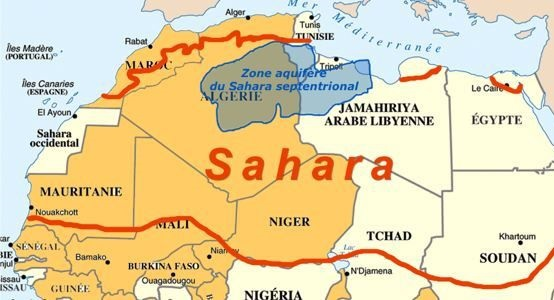
\includegraphics[scale=0.40]{media/zone_aquifere_sahara.jpg}
  \caption{
    Nappe phréatique au Maghreb\newline
      \tiny{Source:\newline
        \url{https://i1.wp.com/www.webdo.tn/wp-content/uploads/2014/03/Carte-photo-canalblog.jpg}
      }
  }
  \label{fig:zone_aquifere_sahara}
\end{SCfigure}

Autre ressource, autre cause de conflit, les terres rares sont inégalement réparties
sur Terre : la Chine possède près de 60\% des réserves mondiales.

\begin{SCfigure}[][h]
  \centering
  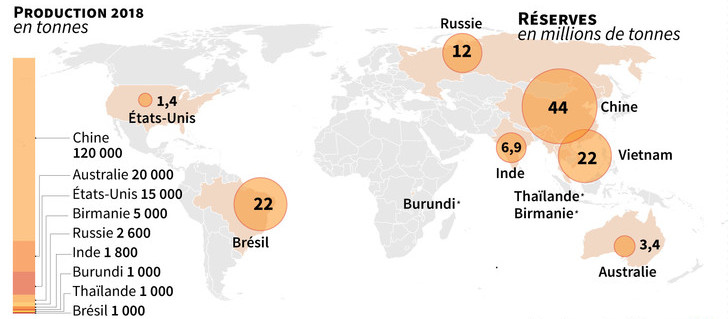
\includegraphics[scale=0.5]{media/terres_rares.jpg}
  \caption{
    Production et réserves de métaux rares\newline
      \tiny{Source:\newline
        \url{https://img.aws.la-croix.com/2019/05/29/1301025438/Production-reserves-metaux-rares_1_728_388.jpg}
      }
  }
  \label{fig:terre_rare}
\end{SCfigure}

\section{Réchauffement climatique}

L'augmentation des besoins des être humains a également une conséquence sur l'environnement.
La production d'énergie et sa consommation entraînent une production de carbone dangereuse pour le maintien de l'équilibre des écosystèmes.
La quantité de Gaz à Effet de Serre - GES - dans l'atmosphère est à la hausse, ce qui sur Terre se traduit par différents impacts :
\begin{itemize}
  \item Augmentation de la température terrestre et dérèglement climatique ;
  \item Fonte glacière et montée des eaux ;
  \item Acidification des océans ;
  \item Disparitions d'espèces animales ;
  \item Augmentation du nombre et de l'intensité des catastrophes naturelles ;
\end{itemize}

\begin{figure}[h]
  \centering
  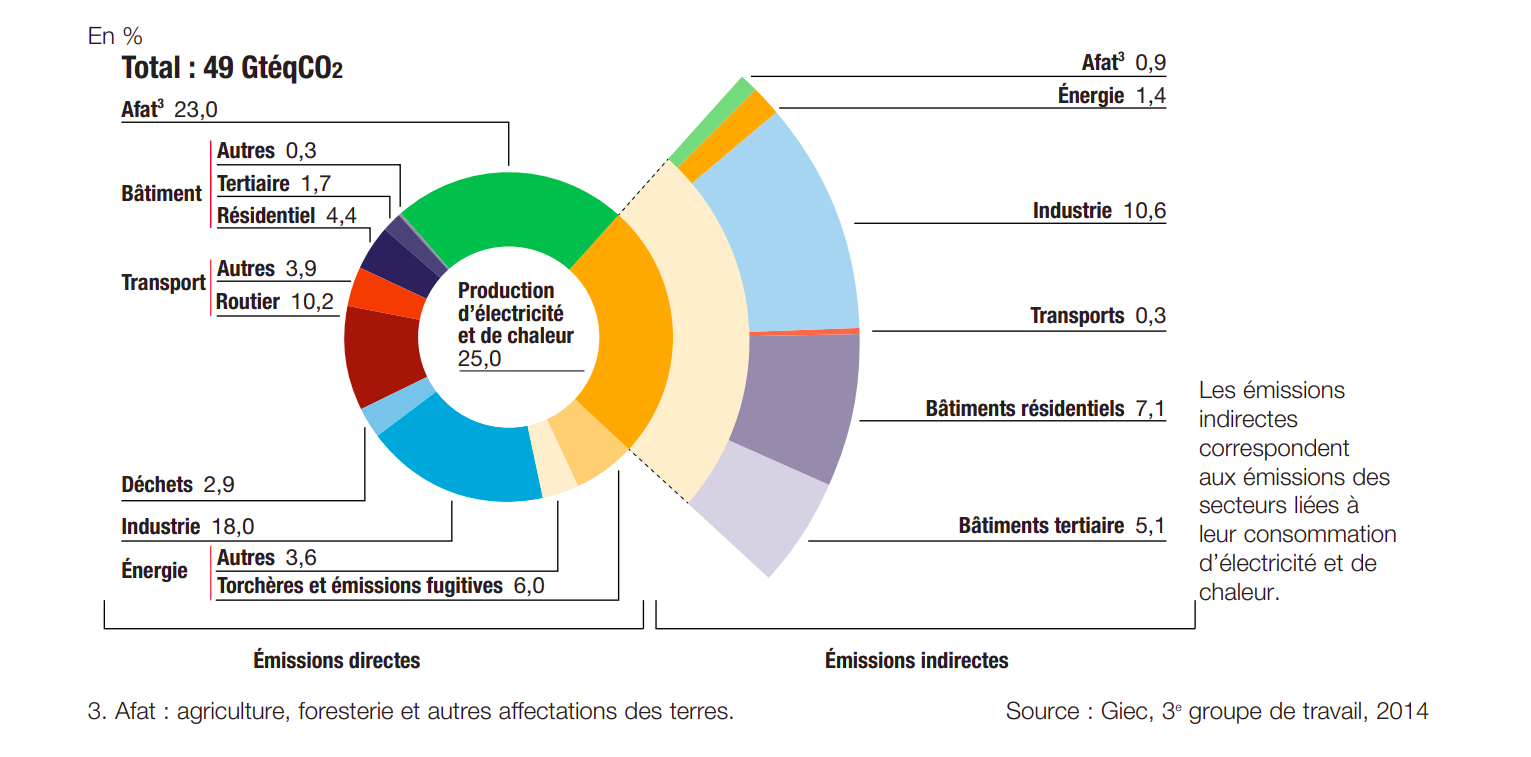
\includegraphics[scale=0.30]{media/repartition_ges.png}
  \caption{ Répartition des émissions mondiales de GES par secteurs en 2010\newline
      \tiny{Source:
        \url{https://www.connaissancedesenergies.org/sites/default/files/pdf-actualites/rep_-_chiffres_cles_du_climat_2016.pdf}
      }
  }
  \label{fig:terre_rare}
\end{figure}

L'Arcep a publié en octobre 2019 une estimation de l'empreinte carbone du numérique.
Elle représenterait 3\% des émissions de GES mondiales.
C'est à la fois une part non négligeable, mais relativement peu quand on le compare au reste de la repartition des émissions mondiales.
Il y a plus à gagner en réduisant nos émissions dans les autres secteurs qu'en essayant de grignoter sur ce 3\%.
La technologie peut en effet être un moyen de limiter le total des autres secteurs en les optimisant.

\section{Amélioration des performances informatiques}

Cette part d'émissions de GES pour le numérique est néanmoins à surveiller.

La technologie est en constante progression depuis toujours et est de plus en plus puissante.
L'augmentation de la vitesse de calcul et du stockage des données ont changé la manière dont l'Homme communique avec la machine.
Il peut parler dorénavant parler en langage naturel à des assistants personnels pour combler ses besoins du quotidien.
Ces besoins nouveaux s'inscrivent dans une dynamique datant de l'ère industrielle qui veut que
la population améliore sa qualité de vie quotidienne.

Grâce à ces performances, un français moyen mène une vie plus confortable qu'un roi du Moyen-Âge.

Cependant, le futur voit une perte de vitesse dans cette augmentation de performance.
Augmenter la complexité des composants davantage n'est plus suffisamment rentable pour renforcer une machine.
Mais l'évolution de la communication entre machines nous permet de contourner cette limite.
Il ne suffit plus de créer des machines sur-performantes, mais de créer un
réseau pour en augmenter le nombre.

% Image montrant l'augmentation de performance

D'autre part, cette augmentation de performance connaît un travers auprès des concepteurs logiciels.
Les services numériques bénéficiant d'outils de plus en plus puissants, le soucis d'optimisation est souvent mis au second plan.
Ils deviennent en effet de plus en plus gourmands et n'hésitent pas à exploiter toute la capacité de la machine sur des fonctionnalités souvent accéssoires.
Le terme d'obésiciels est utilisé pour décrire cette tendance.

\section{Vers une optimisation de l'énergie}

Nous pouvons faire l’analogie avec le développement d'une application logicielle. Une règle courante est d’éviter
l’optimisation prématurée, c’est à dire de ne pas optimiser tant que le besoin ne s’en fait pas
ressentir. Nous risquerions de dépenser du temps et de l'énergie dans quelque chose qui
peut-être ne fonctionne pas comme nous le voudrions.
Dans un premier temps, il faut faire en sorte que le système fonctionne correctement.
On peut préférer la quantité face à la qualité. On ne cherche à optimiser cette méthode
qu’ensuite, lorsque les ressources commencent à ne plus suffire ou qu’un besoin de remise
à l’échelle se fait sentir.

Nous sommes en mesure de produire suffisamment d’énergie pour répondre aux
besoins de la population d'aujourd'hui. Mais le contexte nous impose désormais d’optimiser
nos méthodes : épuisement des énergies fossiles, dérèglement climatique, augmentation de la
population.




